\section{Proposed solution}
Before going into the details of the solution, let's describe the graphs 
used for the analysis. The dataset used is a set of synthetic 
graph generated using the Erdos-Renyi model.
Therefore, the graph generates $ER(n, p)$ is parametric in $p$ and $n$, whereas $n$ is the number of nodes and $p$ can be interpreted formally as the probability
of attaching a node regardless the previous realizations.  On the another hand it
can be seen as the density of the graph. In particular the set used by the experiments
is composed by four different graphs: $ER(10000, 0.2), ER(10000, 0.4), ER(10000, 0.8), ER(100000, 0.002)$. 
The number of nodes was chosen as a tradeoff on a reasonable size, to evaluate the
goodness of the algorithm and the cost in terms of memory and space required, since
the space and time complexity are $O(n^2)$ which are not negligible\footnote{for low density a better algorithm were used provided in the networkx library, that were proposed by Vladimir Batagelj and Ulrik Brandes\cite{PhysRevE.71.036113}}.
\subsection{Problem Analysis}
\subsubsection{Completion time}
\label{sec:comp-time}
The sequential algorithm described in section .\ref{sub:seq-version} is an
iterative algorithm with an initialization phase where the $i$-th iteration visits level $i$. The
processing of the $i$-th level requires to go through each node
$v : d(v, s) = i$ and visit its neighborhood.
The time needed to process a node is independent of the
level at which it is visited as it only depends on the size
of its neighborhood. Hence, let the time taken by the node $v$ be denoted 
with $T_v$. Then the time taken by the level $i$ is $T_{L_i} = \sum_{v : d(v, s) = i}T_v$.
Note that different levels require different times depending on the topology of the graph. In particular, the $i$-th level is influenced by the number of nodes at distance $i$ from the root 
and by the size of the neighborhood of these nodes. The completion time of the $i$-th
iteration is given by $T_i = T_{L_i} + T_{swap} + T_{clear}$, i.e. the time taken by the level $i$ plus two additional factor: the former, $T_{swap}$, is the time taken to swap 
$L$ and $\hat{L}$, which is the same for all the iterations since it is a swap of two pointers; the latter, $T_{clear}$, is
time taken by the cleaning of the new $\hat{L}$ so it depends on number of elements.
Let $G$ be the graph induced by the root node then the completion time for the sequential algorithm is:
$$
T_{seq}(G) = T_{init} + \sum^{\bar{d}(G)}_{i=1} T_i \leq  T_{init} + (\bar{d}(G) \cdot max_i \ T_i)
$$

Where $T_{init}$ is the time taken by the
initialization phase, therefore it takes into account: the initialization of the 
vector of visits, the initialization of $F_i$ and $F_{i+1}$, the analysis 
of the root node, the insertion of its neighbors in the frontier and 
the creation of the vector of visits.

There mainly are three kind of possible parallelism:
\begin{enumerate}
    \item The frontier-level: which divides 
    the work required by the computation of the single frontier among the workers;
    \item The neighborhood-level: which divides the work required by the single
    node computation, hence the visit of its neighbors among the workers;
    \item A combination of both 1 and 2.
\end{enumerate}
The analysis is focused on the first approach since the second
one is very sensitive to the local topology of a single node. 
Moreover, 
in real scenarios $\bar{k}$ is a very small value, which causes small units of work. 
In addition, still considering real scenarios, $\bar{d}$ is a very small number
 and $n$ is a big value, 
whereby the frontiers will contain a very large number of nodes.
\\
\\
Ideally, considering $nw$ workers one could think that the analysis of a single
frontier $F_i$ can be divided equally among the workers, obtaining a parallel
completion time for a single iteration $T^{par}_{T_i} \approx \frac{T_{L_i}}{nw} + T_{swap} + T_{clear}$. 
However, this does not take into account that the analysis of
$L_{i+1}$ can start only when the analysis of $L_{i}$ is terminated,
which causes an additional time factor to synchronize all the workers. 
The parallel completion time for a single iteration becomes then:
$T^{par}_{T_i} \approx \frac{T_{L_i}}{nw} + T_{sync} + T_{swap} + T_{clear}$.
Hence, 
there are three tasks that can not be done concurrently, 
as they are in critical section:
\begin{enumerate}
    \item Checking if a node has already been visited and, in the case it is 
    necessary, updating the vector of visits;
    \item Adding the nodes found to $F_{i+1}$;
    \item Update the number of occurrences.
\end{enumerate}
Lets denote the additional factors listed above with:
 $T_{visited}$ due to 1, $T_{merge}$ due to 2 and $T_{update}$ due to 3.
 The first two are required at each iteration, the last one can be 
 added directly once to $T_{par}$ since each workers
 can keep a counter of the found occurrences and at the end sum it.
 The completion time of single iteration in parallel can be better 
 approximated by: $T^{par}_{T_i} \approx \frac{T_{L_i}}{nw} 
 + T_{sync}
  + T_{visited} + T_{merge} + T_{swap} + T_{clear}$, resulting in the following 
  parallel completion time: 
  $$
  T_{par}(G, nw) \approx T_{init} + T_{update} + \sum^{\bar{d}(G)}_{i=1} T^{par}_{T_i}
  $$



Of course the above approximation considers the workload as perfectly balanced,
that in principle is not easy to achieve, since it is not only
a matter of the number of nodes (i.e. it is not enough to assign equal-size
subset of the frontier to each worker). On the other hand, the completion time $T_{S \subseteq L_i}$
is influenced by the completion time of each node $v \in S$, namely $T_v$. A necessary condition for the best scenario is that at iteration $i$, not necessary the best,
is the one where the number of nodes at level $L_{i+1}$ is equally
distributed among the neighbors of nodes contained in $L_i$.
\subsubsection{Sequential analysis}
In order to design a proper parallel solution, 
the times of the various operations and phases that the sequential
 version requires were measured, to identify if there are any bottlenecks.
The expected ones are the memory accesses, more in detail:
\begin{itemize}
    \item The time to access an element of the graph contained in the frontier,
    $T_{read(v[i]\in G)}$, that is 
    random and unpredictable, since it only depends on the topology of the graph. One could
    imagine that a possible improvement is to sort the frontier, this probably causes
    an overhead that exceeds the gain, however, more 
    considerations require an additional 
    analysis that this work does not take into account.
    \item The same reasoning on accessing graph elements
     also applies to the time to access the vector of visits, $T_{visited[v]}$, where, however, 
    the access order is influenced by the organization of the neighborhood 
    of the nodes in $L_i$.
\end{itemize}
The accesses to the current frontier $F_i$ and the neighborhood $\mathcal{N}(v)$ are efficient, since they are a scan from the 
first to the last elements
of the vector, thus optimal in number of I/Os. Some of
 the measures to support this are presented in Table \ref{tab:seq-meas}\footnote{The results are obtained as an average over 10 runs}. Note the time taken by $T_{read(v \in \mathcal{N}(v))}$, $T_{read(visited[v])}$, $T_{write(visited[v])}$ were not measured since on average they took at most $\approx 5ns$.

\begin{table}[h]
    \begin{center}
        \begin{tabular}{|| l | c | c | c | c |}
            \hline
            & $ER(10000, 0.2)$ & $ER(10000, 0.4)$ & $ER(10000, 0.8)$ & $ER(100000, 0.002)$ \\ \hline \hline
             $T_{clear}$  & $\approx 164ns$& $\approx 176ns$& $\approx 167ns$ & $\approx 155ns$
             \\ \hline 
             $T_{swap}$  & $\approx 154ns$& $\approx 168ns$& $\approx 163ns$ & $\approx 140ns$
             \\ \hline 
             $T_{read(i \in F_i)}$  & $\approx 160ns$& $\approx 164ns$ & $\approx 166ns$ & $\approx 150ns$
             \\ \hline 
             $T_{read(v[i] \in G)}$  & $\approx 1874ns$& $\approx 2837ns$& $\approx 4233ns$ & $\approx 771ns$
             \\ \hline 
             \hline
        \end{tabular}
    \end{center}
    \caption{Sequential  measurements}
    \label{tab:seq-meas}
\end{table}
As can be observed, as the density increases the time taken by the I/O increases. This happens because the bigger is the vector to read the higher is the number of pages it takes in the upper-level cache, i.e. higher is the number of access to those pages for a scan. The sequential completion 
times measured is shown in Table \ref{tab:seq-results} as average on 10 runs.
\begin{table}[!htb]
    \begin{center}
        \begin{tabular}{|| l | c | c | c | c ||}
            \hline
              & $ER(10000, 0.2)$ & $ER(10000, 0.4)$ & $ER(10000, 0.8)$ & $ER(100000, 0.002)$ \\ \hline \hline
             $\bar{T}_{seq}$ & $65ms$ & $126ms$ & $244ms$ & $127ms$ \\ \hline
             $\sigma(T_{seq})$ & $1ms$ & $422\mu s$ & $548\mu s$ & $399 \mu s$ \\ \hline
            \hline
        \end{tabular}
    \end{center}
    
    \caption{Sequential results}
    \label{tab:seq-results}
\end{table}

Considering the results obtained, different scenarios can be explored as interesting for the analysis of the parallel version: for instance a graph having a small number of nodes and fully connected generates a big frontier w.r.t. the number of nodes, although the time needed to process the frontier is too small compared to the overheads of thread creation. Similar scenario happens for processing graph with large number of nodes and really high value of $\bar{d}$ where the frontiers generated in average will be small, thus the overhead in synchronization is expected to exceeds the gain.

\subsection{Solution Description}
In order to prevent the load balancing issues 
due to the variance of $k_{out}$, the proposed solution
uses a dynamic scheduling, which can be easily implemented
in a Master-Worker fashion. In the
present case, an auto-scheduling policy is implemented:  all the workers have access to the frontier
and obtain a new task of work using a shared
data structure. Retrieving a task has the cost of an
atomic fetch+add on an integer. Here a task correspond to a chunk, i.e.
 start and end indexes of $F_i$. Note that the size of the chunk $cw$
 is a parameter of the solution. Thanks to this shared data structure
 the master does not need to
 prepare the tasks for the workers. Instead it performs the same work as 
 the worker with the difference that is also responsible for 
 the swap and the cleaning of the new $F_{i+1}$. 
\subsubsection{Local next frontier}
The trivial way to produce $F_{i+1}$ is to share an array among the workers and insert each new element in mutual exclusion, each new element found to the array. This solution is as easy as inefficient, since it produces different problems. First of all, false sharing occurs more frequently and the overhead due the atomicity is really high. In the proposed solution each worker has a local version of $F_i$, which contains only the nodes found by the worker at the end of the visit. The worker atomically adds all the elements of the local frontier to the global one. This reduces false sharing and decreases the overhead, since the processing is much faster.  
\subsubsection{Expected performance}
\label{sec:how-it-perform}
The solution mentioned above mitigates, thanks to dynamic scheduling,
the problems due to the variance of $k_{out}$.
However, it does not eliminate the
problem in its entirely, because it remains 
a parallelism only at the frontier level.
The worst case is when an huge hub occurs: 
since the worker who has to process it,
will take much longer.
\\
\\
To discuss with more specificity the expected performance, it is necessary to evaluate it with respect to the topology and statistical properties of the input graph:
\begin{itemize}
    \item In general, the lower the value of $\bar{d}$ is, the higher the expected gain of the parallel version, because the overhead due to the level-synchronization will be the smaller and, the number of nodes in the frontiers will be higher, since $n$ should be divided among few frontiers.
    \item In addition, fixing $\bar{d}$ and enlarging $n$ increase the probably that some levels will contain a number of nodes high enough to achieve a good speedup increase.
    \item In addition to the previous property, if the $k_{out}$ is considered, it is possible to better estimate how the frontiers will be made. Namely, as the variance in $k_{out}$ is low, the confidence in the fact the nodes between the frontiers will be better distributed increases. This is not true in general, because actually it depends on which node are present in the different neighborhoods: the fewer are the duplicates among the nodes neighborhood the better distributed the nodes will be across the frontiers.
    \item Instead, the density itself does not say too much about about the distribution of the nodes among the levels, but in some specific case it can helps. For instance the synthetic dataset generated through the Erdos-Renyi increasing the value of $p$, i.e. the density, the algorithm tends to generate a small number of levels due to independency in drawing random edges: for small value of p the probability of finding node in higher level increases.

\end{itemize}

For example, in real graphs it is known that $n$ is a big number and $\bar{d}$ is really small number. Even though in those graphs hubs occurs often and this generates an high variance in $k_{out}$ and increments the load balancing issue.

\subsubsection{The influence of chunksize}
\label{sec:chunksize}
As mentioned before the proposed solution is parametric in $cw$, namely the chunksize, this measure refers to the number of nodes of $F_i$ that each workers will consider as a single task. The pop operation is as written in the previous sections with an efficient data structure that implements it at the cost of an atomic \texttt{fetch-add}. The choice of $cw$ value should be a trade-off between the advantage of having small tasking and the time taken by the pop operation. Small chunk size guarantees a fairer distribution among the workers, as cons it increments the number of pops, hence the overhead. Moreover if the expected variance in $k_{out}$ is high the advantage of having small chunk increase.
\subsection{Analysis and measurements}
All the experiments have been performed fixing $cw$ as 32, this number has been chosed according to what is written in section \ref{sec:chunksize} observing the overhead better described in section \ref{sec:overhead}.
\subsubsection{Build and execution}
The source code have been complied with \texttt{g++17} using the commands:
\begin{itemize}
    \item \texttt{g++ -std=c++17  ./src/bfs-sequential.cpp -o ./build/bfs-sequential -O3} \\ \texttt{-Wall -I include/ -ftree-vectorize }
    \item \texttt{g++ -std=c++17  ./src/bfs-pthread.cpp -o ./build/bfs-pthread -O3 -Wall} \\ \texttt{-pthread -I include/ -ftree-vectorize }
    \item \texttt{g++ -std=c++17  ./src/bfs-fastflow.cpp -o ./build/bfs-fastflow -O3 -Wall}\\ \texttt{-pthread -I include/ -ftree-vectorize }
\end{itemize}
The execution of the sequential code requires 3 positional arguments:
\begin{enumerate}
    \item \texttt{inputFile} : string, the path to the graph
    \item \texttt{startingNodeId} : integer, the id of the from which the bfs will start
    \item \texttt{labelTarget} : integer, label whose occurrences are to be counted
\end{enumerate}
The parallel versions requires 2 additional positional arguments:
\begin{enumerate}
    \item \texttt{nw} : integer, the number of workers to use
    \item \texttt{k}: integer, chunk size
\end{enumerate}
All the version print by default the completion time.
\subsubsection{pthread implementation}
In the \texttt{pthread} implementation, the main thread acts as master and so, 
it executes the initialization phase, creates 
the threads and then starts its work as described. As soon as the visit of the graph
is completed the master collects the result and prints it together with the completion time. The synchronization at the end of each level, among the workers and the master, 
is implemented using an active wait barrier implemented through mutex and conditional variable.
\\
To handle the critical section in the check and update of the visited nodes a vector of atomic booleans was used as the vector of visits. The check and update was accomplished via a \texttt{compare and exchange} instruction, which was done at the node level in the frontier. Meanwhile at the neighborhood level (the one implemented in the sequential version) to avoid inserting duplicates a non-atomic vector of boolean was used, namely the \textit{vector of insertion}. Since the vector of insertion is composed by non-atomic boolean this does not guarantee that duplicates will not be added, but the checks at node level guarantee that the node will not be visited more than once. This was made because the vector of insertion generates few duplicates in the frontier the checks at node level will have often the same result, hence this helps to exploiting better the pipeline of the new processor through the branch prediction. The probability of adding duplicates grows as the $C(v)$ of the nodes $v$ in the previous frontier increase. A downside of the introduction of this vector is that it increases the probability that false sharing occurs. 
\subsubsection{Overhead analysis}
\label{sec:overhead}
To better evaluate the performance as the number of threads increases, it is useful to observe the trend that the overheads show. With this type of analysis it is also possible to make a choice on the effective number of threads to use in case the nature (e.g. using the approximation of the completion time provided in section \ref{sec:comp-time}), intended as topology and statistical properties, of the graph is known. Two three classes of overhead can be identified: 
\begin{enumerate} 
    \item the first class grows linearly in the number of thread, which contains the creation of the threads $\bar{T}_{thd}$.
    \item the second class grows linearly in the $\bar{d}$ (the number of frontier): the synchronization time and the waiting for the lock, $T_{merge}$.
    \item the third class instead depends on the size of $F_i$, which contains: the overhead to checks and update atomically, $T_{visit}$, the vector of visits and the one needed to pop a new task, $T_{pop}$.
\end{enumerate}

\begin{table}[!htb]
    \begin{center}
        \begin{tabular}{|| l | c ||}
            \hline
             $T_{thd}$ & $130 \mu s$  \\ \hline
             $T_{visited}$ & $280ns$ \\ \hline
             $T_{pop}$ & $480ns$ \\ \hline
            \hline
        \end{tabular}
    \end{center}
    

    \label{tab:static-overhead-results}
    \caption{Static overhead measurements}
\end{table}

Even though the synchronization belongs to the second class, its value depends on the number of threads as shown in figure \ref{fig:level-sync}. The same applies to $T_{merge}$, the lock waiting, for which it also depends on the size of the local frontiers. Its trend is non-trivial as shown in figure \ref{fig:lock}: if the number of threads grows the overhead increases, in any case if the generated local frontiers are small as in the case of Erdos-Renyi with low density the growth decreases.

\begin{figure}[!htb]
    \centering
    \begin{minipage}{0.48\textwidth}
        \includegraphics[width=\textwidth]{plots/level-sync.pdf}
        \caption{Level-synchronization overheads}
        \label{fig:level-sync}
    \end{minipage}
    \begin{minipage}{0.48\textwidth}
        \includegraphics[width=\textwidth]{plots/lock-wait.pdf}
        \caption{Lock overheads}
        \label{fig:lock}
    \end{minipage}
\end{figure}

\subsubsection{Fastflow implementation}
The \texttt{FastFlow} version implements the same mechanisms as in the \texttt{pthread} version, except for the synchronization mechanisms, since it uses the Master-Worker with feedback queue. The master after having performed the initialization phase and indicated to the threads which is the pointer to the queue where to write the nodes they find, performs the same work of the workers and orchestrates the level-synchronization. The level-synchronization is implemented through the task queues and feedback queue, that were used to notify the master with the number of occurrences found in the level. Whenever the master receives all the feedbacks from all the workers, it swaps the pointers of $F_i$ and $F_{i+1}$ and informs the threads to work on the next level by indicating the new pointers pushing them on the task queues of each worker. Initially to start the worker the master pushes the initial pointers on the task queues.
\subsubsection{Results}
The following section reports all the results obtained by both the \texttt{pthread} and the \texttt{FastFlow} implementation. All the synthetic dataset have been exploited in order to show empirically what has been discussed until now. The results have been shown plotting the performances in terms of completion time and speedup reached. The results obtained by the 
\texttt{FastFlow} version are worse in general than the \texttt{pthread} implementation. The gap shows an increasing trend as the number of threads grows. This gap is probably due to the fact that the \texttt{pthread} version can be more specific and implement the bare minimum in a more efficient way for the specific problem, especially in the synchronization mechanisms. 
\\
As discussed earlier as the number of nodes in the frontiers increases, an increase in speedup is expected. In the Erdos-Renyi model fixed the number of nodes $n$, as $p$ increases we obtain graphs with a smaller number of frontiers, i.e. $\bar{d}$ smaller, and generating very large frontiers. This is well highlighted comparing the different plots in Figures
\ref{fig:perf_02}, \ref{fig:perf_04} and \ref{fig:perf_08}. Interestingly, as the number of nodes in the frontiers increases and, the number of frontiers decrease (because $n$ is fixed), the gap between the performances of the two versions shows a decreasing trend.

\begin{figure}[!htb]
    \centering
    \begin{minipage}{0.48\textwidth}
        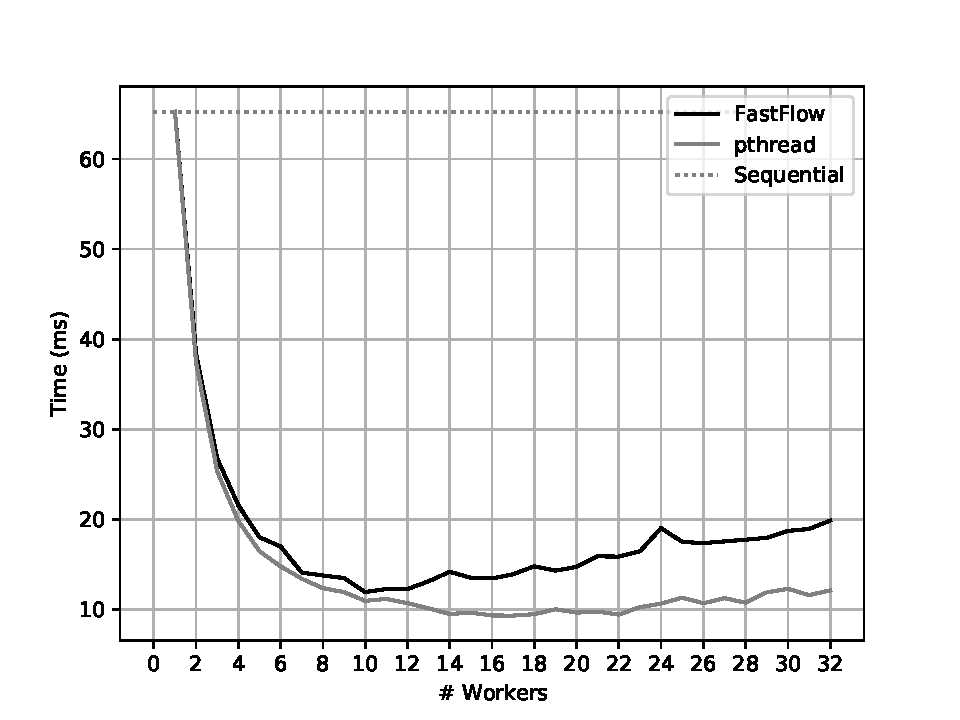
\includegraphics[width=\textwidth]{plots/fastflow_performance_02_time.pdf}
    \end{minipage}
    \begin{minipage}{0.48\textwidth}
        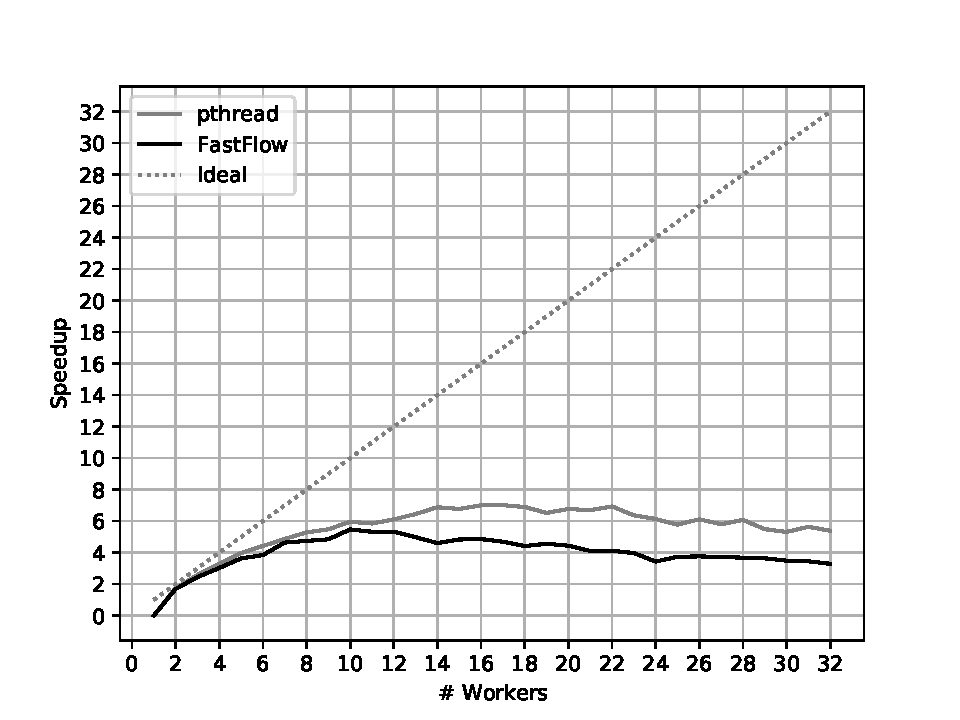
\includegraphics[width=\textwidth]{plots/fastflow_speedup_02_time.pdf}
    \end{minipage}
    \caption{Performance and speedup using ER(10000, 0.2)}
    \label{fig:perf_02}
    \begin{minipage}{1\textwidth}
    \end{minipage}
    \begin{minipage}{0.48\textwidth}
        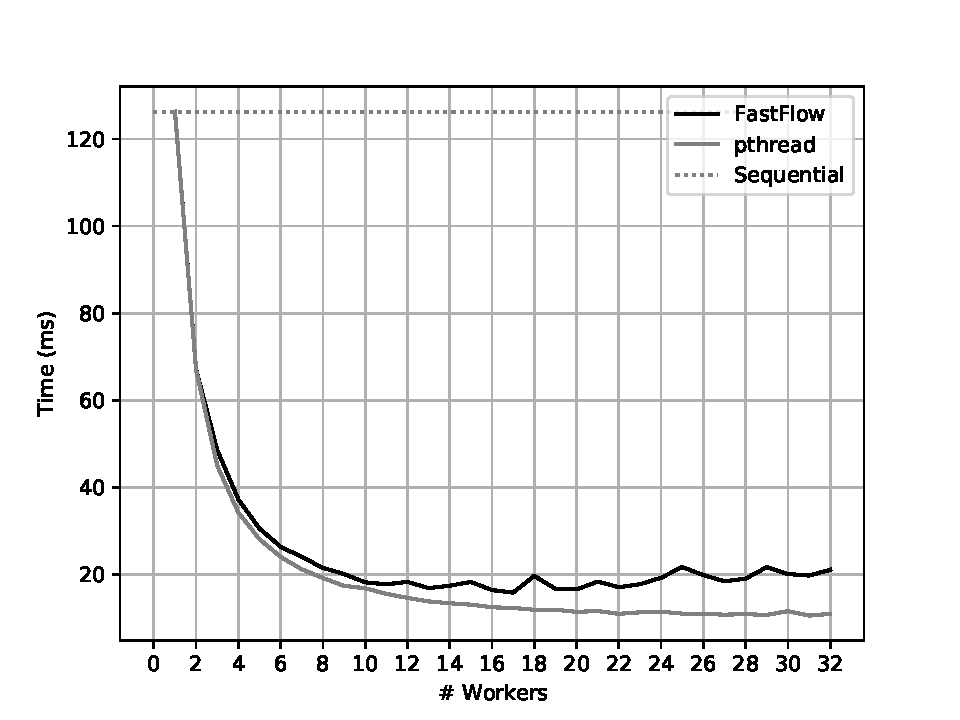
\includegraphics[width=\textwidth]{plots/fastflow_performance_04_time.pdf}
    \end{minipage}
    \begin{minipage}{0.48\textwidth}
        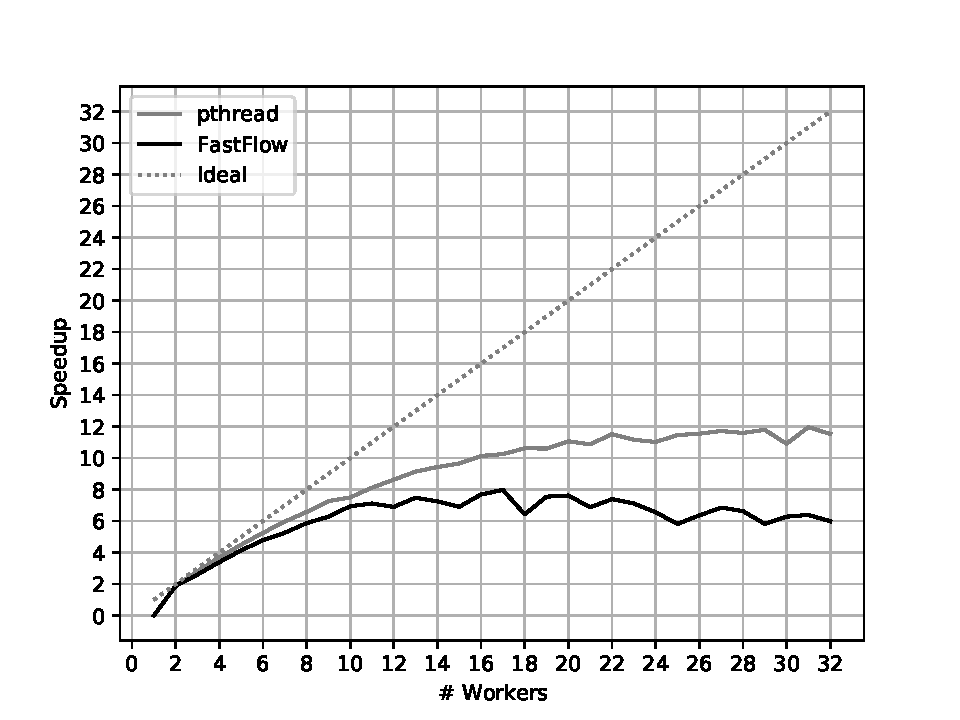
\includegraphics[width=\textwidth]{plots/fastflow_speedup_04_time.pdf}
    \end{minipage}
    \caption{Performance and speedup using ER(10000, 0.4)}
    \label{fig:perf_04}
    \begin{minipage}{1\textwidth}
    \end{minipage}
    \centering
    \begin{minipage}{0.48\textwidth}
        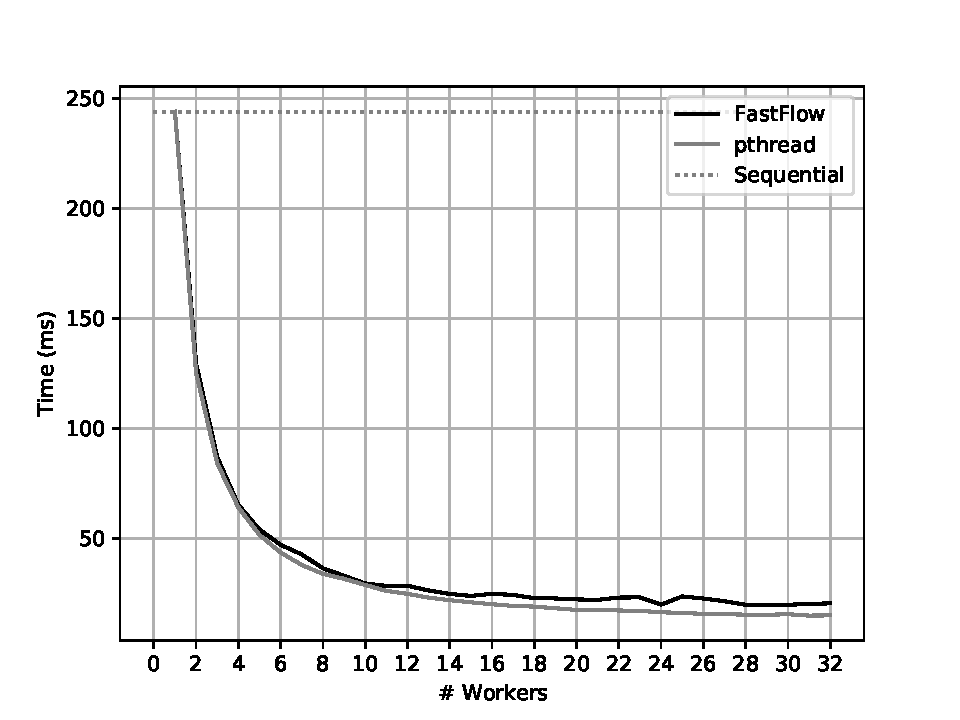
\includegraphics[width=\textwidth]{plots/fastflow_performance_08_time.pdf}
    \end{minipage}
    \begin{minipage}{0.48\textwidth}
        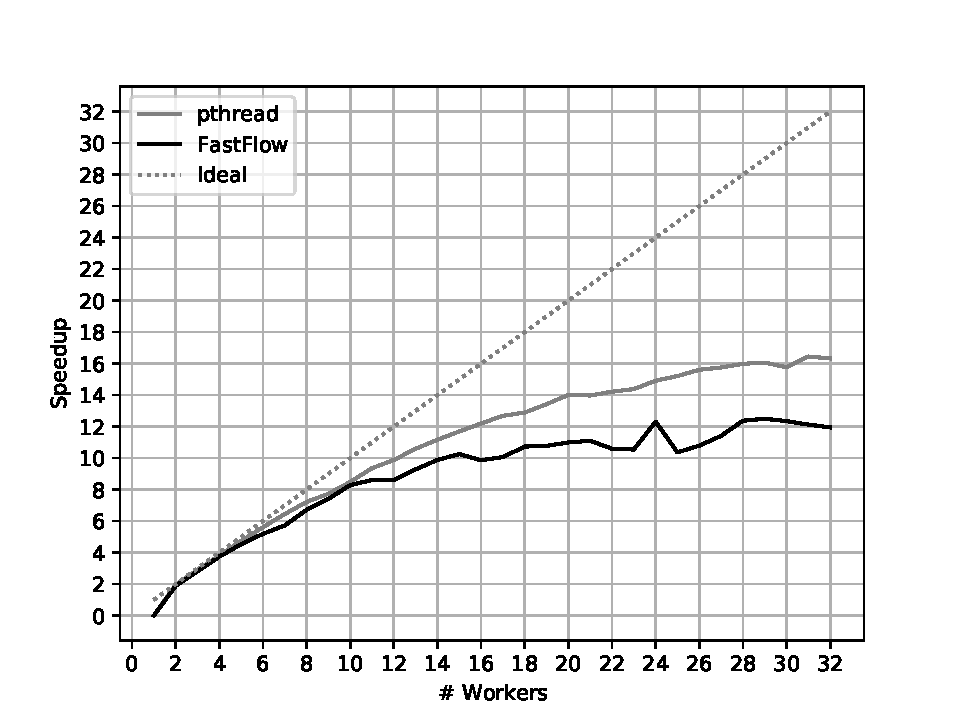
\includegraphics[width=\textwidth]{plots/fastflow_speedup_08_time.pdf}
    \end{minipage}
    \caption{Performance and speedup using ER(10000, 0.8)}
    \label{fig:perf_08}
\end{figure}

Moreover, as mentioned in section \ref{sec:how-it-perform} it is not only a matter of density, instead different factors must be taken into account, such as the number of nodes and $\bar{d}$. This is clear looking at the result obtained in Figure \ref{fig:perf_08} and \ref{fig:real-case}.

\begin{figure}[h]
    \centering
    \begin{minipage}{0.48\textwidth}
        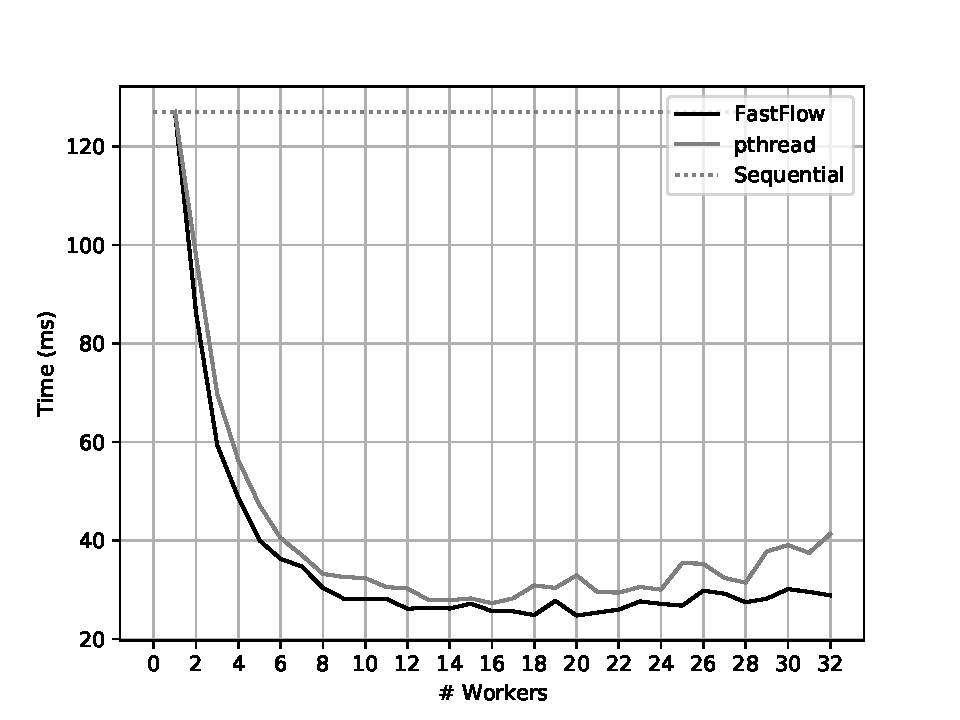
\includegraphics[width=\textwidth]{plots/fastflow_performance_002_time.pdf}
    \end{minipage}
    \begin{minipage}{0.48\textwidth}
        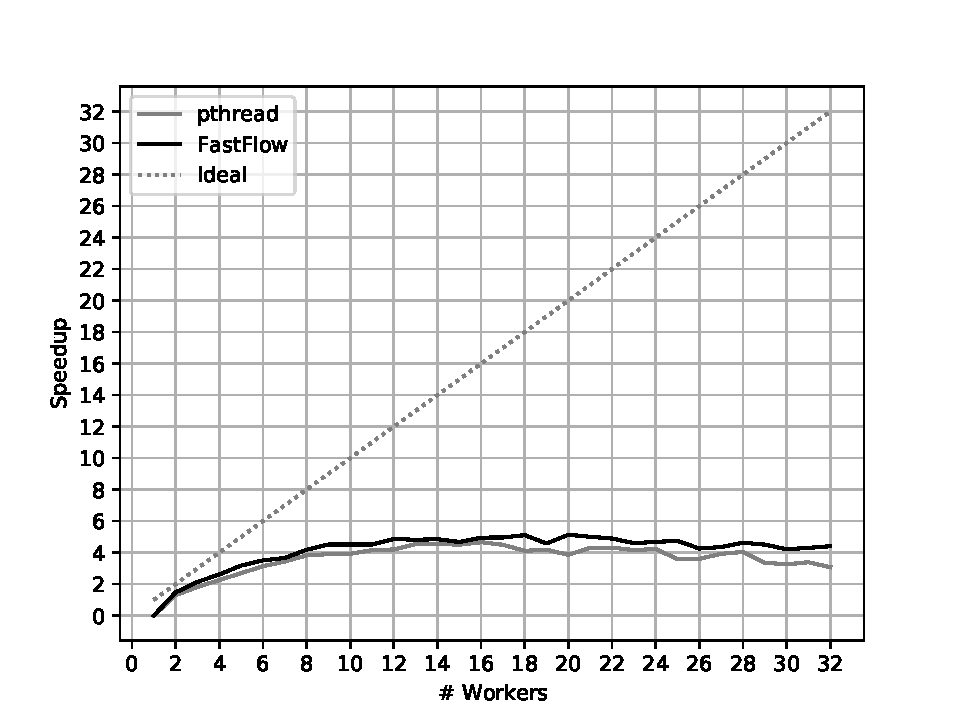
\includegraphics[width=\textwidth]{plots/fastflow_speedup_002_time.pdf}
    \end{minipage}
    \begin{minipage}{1\textwidth}
    \caption{Performance and speedup using ER(100000, 0.002)}
    \label{fig:perf_002}
\end{minipage}
\end{figure}
\subsection{A real use case}
To further evaluate the solutions, a real case is shown, using as
 input a real network of $149279$ nodes and $\approx 10530774$ edges, hence $0.00095$ as density. The 
 network was built as a network
  of interactions happened in the 
  month of october 
 2020 in the /r/politics subreddit. The nodes represent users who have 
 commented or written posts, while the edges from user 
 A to user B indicates that the former has posted a comment to the latter. 
 The results obtained are reported in terms of performance and speedup in 
 the Figure  \ref{fig:real-case}.

\begin{figure}[h]
\centering
\begin{minipage}{0.48\textwidth}
    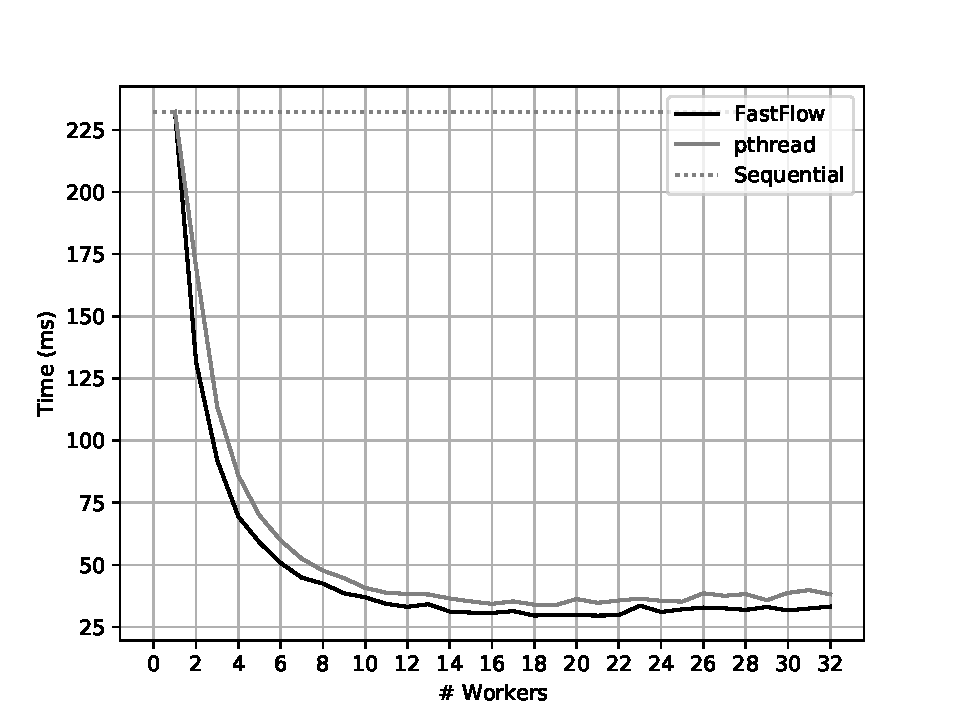
\includegraphics[width=\textwidth]{plots/fastflow_performance_real_time.pdf}
\end{minipage}
\begin{minipage}{0.48\textwidth}
    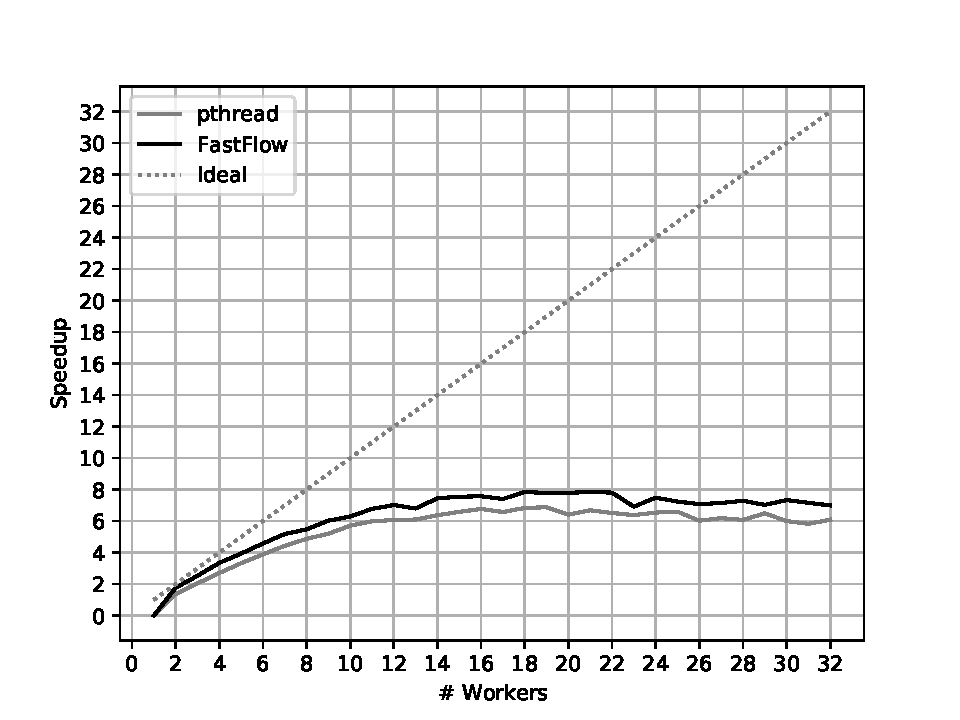
\includegraphics[width=\textwidth]{plots/fastflow_speedup_real_time.pdf}
\end{minipage}
\caption{Real use case speedup}
\label{fig:real-case}
\end{figure}
